%----------------------------------------------------------------------------------------
%	Packages
%----------------------------------------------------------------------------------------

\documentclass[11pt]{diazessay} % Font size (can be 10pt, 11pt or 12pt)

%----------------------------------------------------------------------------------------
%	Title
%----------------------------------------------------------------------------------------

\title{\textbf{Motion of Three Bodies in Space}} % Title and subtitle
\author{\textbf{Taylor Larrechea} \\ \textit{Colorado Mesa University}} % Author and institution
\date{October 31, 2019} %Date

%----------------------------------------------------------------------------------------
%	Begin Document
%----------------------------------------------------------------------------------------

\begin{document}
\maketitle % Print the title section

%----------------------------------------------------------------------------------------
%	Abstract
%----------------------------------------------------------------------------------------

\begin{abstract}
This Halloween, come witness the mysterious motion of Newtonian Gravitation describing the dynamics of ternary star systems in our universe! Numerical methods were used to solve the governing differential equations, specifically a Forward Euler Difference Scheme for ternary star systems. With the exception of a few very specific systems, it was determined that these star systems are chaotic and unpredictable in their nature.
\end{abstract}

%----------------------------------------------------------------------------------------
%	Document
%----------------------------------------------------------------------------------------
\begin{center}
\begin{figure}[htpb]
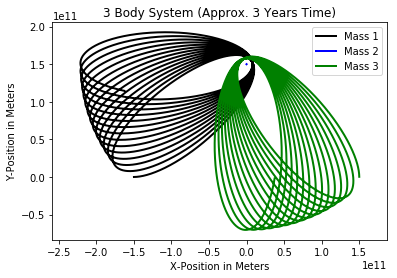
\includegraphics[width=1.00\linewidth]{Figures/3BodyDynamics.png}
\end{figure}
\end{center}
\end{document}

%----------------------------------------------------------------------------------------
%	Comment Headers
%----------------------------------------------------------------------------------------

%----------------------------------------------------------------------------------------
%	
%----------------------------------------------------------------------------------------